\documentclass[xcolor=svgnames]{beamer}
\usepackage[utf8]{inputenc}
\usepackage[english]{babel}
\usepackage{tikz}
\usepackage{pgfplots}

\usetheme{Proso}

\title[Adaptive Practice]{Adaptive Practice of Facts in Domains with Varied Prior Knowledge}
\author{Jan Papoušek}
\institute{Masaryk University Brno}
\date{\today}

\begin{document}
% --------------------------- SLIDE --------------------------------------------
\frame[plain]{\titlepage}
% ------------------------------------------------------------------------------
% --------------------------- SLIDE --------------------------------------------
\begin{frame}
	\frametitle{slepemapy.cz}
	\begin{columns}
		\column{.45\textwidth}
			\includegraphics[width=\textwidth]{2014-IA068-adaptive-practice/africa-with-scale.png}
		\column{.55\textwidth}
			\begin{itemize}
				\item items
					\begin{itemize}
						\item countries
						\item cities
						\item regions
						\item \ldots
					\end{itemize}
				\item users
			\end{itemize}

			\bigskip

			\begin{itemize}
				\item questions
					\begin{itemize}
						\item Select the given place on the map.
						\item What is the name of the highlighted place?
					\end{itemize}
			\end{itemize}
	\end{columns}
\end{frame}
% ------------------------------------------------------------------------------
% --------------------------- SLIDE --------------------------------------------
\begin{frame}
	\frametitle{Assumptions}
	\begin{columns}
		\column{.45\textwidth}
			\includegraphics[width=\textwidth]{2014-IA068-adaptive-practice/africa-with-scale.png}
		\column{.55\textwidth}
			\begin{itemize}
				\item different users have different levels of prior knowledge
				\item different items have different difficulty
				\item if different users sorted items by difficulty,
							the ordering would be similar
			\end{itemize}
	\end{columns}
\end{frame}
% ------------------------------------------------------------------------------
% --------------------------- SLIDE --------------------------------------------
\begin{frame}
	\frametitle{Main Parts}
	\begin{enumerate}
		\item estimation of prior knowledge
			\begin{itemize}
				\item doesn't change or changes very slowly
				\item used for the first answer (student, item)
				\item $\Theta$ -- prior knowledge (every student)
				\item $b$ -- difficulty (every item)
			\end{itemize}
		\item estimation of current knowledge
			\begin{itemize}
				\item evolves during the practice
				\item used for other answers (student, item)
				\item $\bar{\Theta}$ -- current knowledge (student, item)
					\begin{itemize}
						\item initialization: $\bar{\Theta} := \Theta - b$
					\end{itemize}
			\end{itemize}
		\item question selection
	\end{enumerate}
\end{frame}
% ------------------------------------------------------------------------------
% --------------------------- SLIDE --------------------------------------------
\begin{frame}
	\frametitle{Logistic Function: Introduction}
	\begin{center}
		$sig(x) = \frac{1}{1+e^{-x}}$
		\begin{columns}
			\column{0.5\textwidth}
				\begin{center}
					$P(correct|\Theta, b) = sig(\Theta - b)$
				\end{center}
			\column{0.5\textwidth}
				\begin{center}
					$P(correct|\bar{\Theta}) = sig(\bar{\Theta})$
				\end{center}
		\end{columns}
		\begin{tikzpicture}[scale=0.7]
			\begin{axis}[xlabel=$x$, ylabel=$sig(x)$, ymin=0, ymax=1]
				\addplot[blue, domain=-3:3] {1/(1 + exp(-x))};
			\end{axis}
		\end{tikzpicture}
	\end{center}
\end{frame}
% ------------------------------------------------------------------------------
% --------------------------- SLIDE --------------------------------------------
\begin{frame}
	\frametitle{Prior Knowledge: Rasch}
	\begin{itemize}
		\item widely used model
		\item assumes the skill and the difficulty do not change in time
		\item estimation done via \alert{joint maximum likelihood} method
			\begin{itemize}
				\item fixes skills/difficulties $\Rightarrow$ fitting
				\item the whole set of data points is needed
			\end{itemize}
	\end{itemize}
\end{frame}
% ------------------------------------------------------------------------------
% --------------------------- SLIDE --------------------------------------------
\begin{frame}
	\frametitle{Prior Knowledge: Elo}
	\begin{itemize}
		\item used for estimation of skill for chess players
			\begin{itemize}
				\item player -- student/item
				\item match -- question
			\end{itemize}
		\item does not assume the skill and difficulty are constant
	\end{itemize}

	\bigskip

	\hrule

	\begin{center}
		$\Theta := \Theta + K \cdot \left(Result - P(correct|\Theta, b)\right)$

		\medskip

		$b := b - K \cdot \left(Result - P(correct|\Theta, b)\right)$
	\end{center}
\end{frame}
% ------------------------------------------------------------------------------
% --------------------------- SLIDE --------------------------------------------
\begin{frame}
	\frametitle{Prior Knowledge: Rasch vs. Elo}
	\begin{center}
		\includegraphics[width=0.8\textwidth]{2014-IA068-adaptive-practice/elo-rasch-comparison.png}
	\end{center}
\end{frame}
% ------------------------------------------------------------------------------
% --------------------------- SLIDE --------------------------------------------
\begin{frame}
	\frametitle{Prior Knowledge: Elo Stability}
	\begin{center}
		\includegraphics[width=0.8\textwidth]{2014-IA068-adaptive-practice/elo-history.png}
	\end{center}
\end{frame}
% ------------------------------------------------------------------------------
% --------------------------- SLIDE --------------------------------------------
\begin{frame}
	\frametitle{Prior Knowledge: One Skill?}
	\begin{center}
		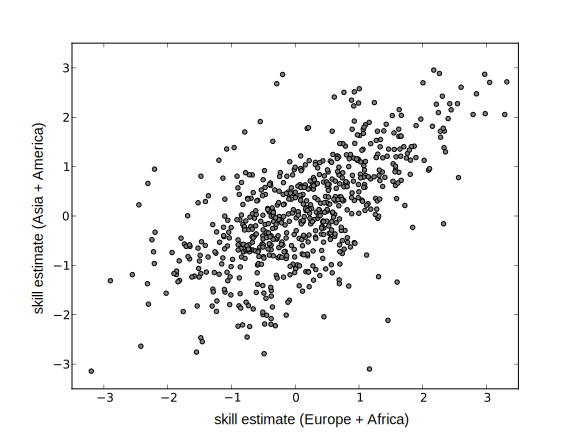
\includegraphics[width=0.8\textwidth]{2014-IA068-adaptive-practice/subskills.png}
	\end{center}
\end{frame}
% ------------------------------------------------------------------------------
% --------------------------- SLIDE --------------------------------------------
\begin{frame}
	\frametitle{Prior Knowledge: Is the difficulty needed?}
	\begin{center}
		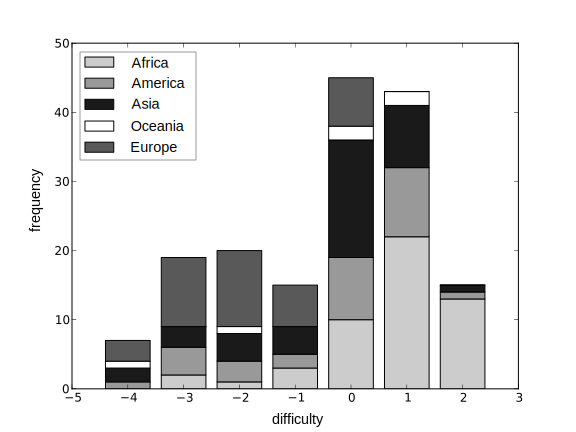
\includegraphics[width=0.8\textwidth]{2014-IA068-adaptive-practice/hist-states.png}
	\end{center}
\end{frame}
% ------------------------------------------------------------------------------
% --------------------------- SLIDE --------------------------------------------
\begin{frame}
	\frametitle{Current Knowledge: Learning Factor Analysis}
	\begin{itemize}
		\item student's knowledge is better with every answer
		\item all answers are equal
	\end{itemize}

	\bigskip

	\hrule

	\begin{center}
		\Large
		$\bar{\Theta} = \bar{\Theta}_0 + \gamma \cdot N_{all}$
	\end{center}
\end{frame}
% ------------------------------------------------------------------------------
% --------------------------- SLIDE --------------------------------------------
\begin{frame}
	\frametitle{Current Knowledge: Performance Factor Analysis}
	\begin{itemize}
		\item student's knowledge changes with every answer
		\item correct answers differ from incorrect answers
		\item the order of answers \textbf{is not} important
	\end{itemize}

	\bigskip

	\hrule

	\begin{center}
		\Large
		$\bar{\Theta} = \bar{\Theta}_0 + \alpha \cdot N_{correct} + \beta \cdot N_{incorrect}$
	\end{center}
\end{frame}
% ------------------------------------------------------------------------------
% --------------------------- SLIDE --------------------------------------------
\begin{frame}
	\frametitle{Current Knowledge: PFAE}
	\begin{itemize}
		\item student's knowledge changes with every answer
		\item correct answers differ from incorrect answers
		\item the order of answers \textbf{is} important
		\item inspired by Elo
	\end{itemize}

	\bigskip

	\hrule

	\begin{description}
		\item[correct]
			$\bar{\Theta} = \bar{\Theta} + \alpha \cdot \left(1 - P(correct|\bar{\Theta})\right)$
		\item[incorrect]
			$\bar{\Theta} = \bar{\Theta} + \beta \cdot \left(0 - P(correct|\bar{\Theta})\right)$
	\end{description}
\end{frame}
% ------------------------------------------------------------------------------
% --------------------------- SLIDE --------------------------------------------
\begin{frame}
	\frametitle{Current Knowledge: Evaluation}
	\begin{center}
		\begin{tabular}{lrrr}
			\textbf{model} & \textbf{RMSE} & \textbf{LL} & \textbf{AUC} \\
			PFA & 0.265 & -44740 & 0.669 \\
			PFA + time & 0.262 & -43088 & 0.695 \\
			PFAE & 0.262 & -41947 & 0.682 \\
			PFAE + time & 0.259 & -40623 & 0.714
		\end{tabular}
	\end{center}
\end{frame}
% ------------------------------------------------------------------------------
% --------------------------- SLIDE --------------------------------------------
\begin{frame}
	\frametitle{Question Selection: Candidate}
	\begin{center}
		\includegraphics[width=\textwidth]{2014-IA068-adaptive-practice/score-functions.png}
	\end{center}
\end{frame}
% ------------------------------------------------------------------------------
% --------------------------- SLIDE --------------------------------------------
\begin{frame}
	\frametitle{Logistic Function: Guessing}
	\begin{center}
		$sig_g(x) = g + (1 - g) \cdot sig(x)$

		\bigskip

		\begin{tikzpicture}[scale=0.7]
			\begin{axis}[xlabel=$x$, ylabel=$sig_g(x)$, ymin=0, ymax=1]
				\addplot[blue, domain=-3:3] {0.4 + 0.6 * (1/(1 + exp(-x)))};
				\addplot[red, domain=-3:3, dashed] {0.4};
			\end{axis}
		\end{tikzpicture}
	\end{center}
\end{frame}
% ------------------------------------------------------------------------------
% --------------------------- SLIDE --------------------------------------------
\begin{frame}
	\frametitle{Question Selection: Options}
	\begin{itemize}
		\item target probability $P_{target} = 0.75$
		\item it is possible to make the question easier by options
			\begin{itemize}
				\item number of options $\sim$ $\frac{1}{g}$
			\end{itemize}
	\end{itemize}

	\bigskip

	\hrule

	\begin{center}
		\Large
		$g = \frac{P_{target} - P_{estimated}}{1 - P_{estimated}}$
	\end{center}

\end{frame}
% ------------------------------------------------------------------------------
% --------------------------- SLIDE --------------------------------------------
\begin{frame}
	\frametitle{Future Work}

	\begin{itemize}
		\item evaluation of question selection
			\begin{itemize}
				\item we want to optimize learning
			\end{itemize}
		\item deal with estimation uncertainty
			\begin{itemize}
				\item useful for new users and new items
			\end{itemize}
		\item map recommendation
		\item application in other domains
			\begin{itemize}
				\item vocabulary
				\item anatomy
				\item \ldots
			\end{itemize}
	\end{itemize}
\end{frame}
% ------------------------------------------------------------------------------
% --------------------------- SLIDE --------------------------------------------
\begin{frame}
	\begin{center}
		\Huge QUESTIONS?
	\end{center}
\end{frame}
% ------------------------------------------------------------------------------
\end{document}
